\chapter{Statistiques}
Le logiciel FactDev génère des statistiques tel que le chiffre d'affaire que génère un Client ou un projet. D'autres statistiques peuvent également être obtenues. 
\section{Calcul du Chiffre d'Affaires d'une période\index{Statistiques!Chiffre d'affaire}}
Il est possible d'obtenir le chiffre d'affaire durant une période en cliquant sur le menu << Statistisques $\rightarrow$ Calculer le chiffre d'affaire d'une période >>. La fenêtre ci-dessous s'ouvre:
\begin{figure}[H]
	\centering
	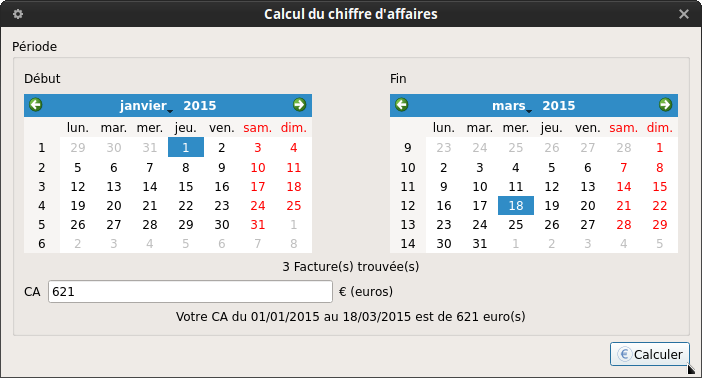
\includegraphics[width=10cm]{screens/calculCAperiode.png}
	\caption{Calculer le Chiffre d'affaire d'une période}
	\label{fig:calculerCAperiode}
\end{figure}

